\documentclass[11pt,a4paper]{article}

\usepackage[margin=1in]{geometry}
\usepackage{lmodern}
\usepackage[T1]{fontenc}
\usepackage{microtype}
\usepackage{booktabs}
\usepackage{parskip}
\usepackage{enumitem}
\usepackage[hidelinks]{hyperref}
\usepackage{titling}
\usepackage{xcolor}

\setlength{\droptitle}{-2.5em}
\setlist{topsep=2pt,itemsep=1pt,parsep=2pt}

\title{\Large FinXplain: Changelog of Paper and Code Revisions \\[2pt]
       \large Post-Defense-Panel Iteration}
\author{Ashton Stephonie T.\ Matias \\
        BS Computer Science, UP Los Ba\~{n}os}
\date{April 29, 2026}

\begin{document}

\maketitle
\thispagestyle{empty}

\section*{1. Context}

This changelog documents the revisions made to the FinXplain manuscript
(\texttt{SP2\_Matias\_journal.tex}) and supporting codebase in response to
defense-panel feedback. The panel raised three concerns:

\begin{enumerate}
    \item The original feature set could not differentiate
    \texttt{maya\_savings} from \texttt{gcash\_gsave}; an additional
    discriminator was needed.
    \item More PSA-derived variables relevant to Filipino financial
    behavior should be incorporated.
    \item A practising financial advisor should be consulted on the
    substantive content of the recommendations.
\end{enumerate}

The changes below address (1) and (2) directly through three new variables
(\texttt{primary\_ewallet}, \texttt{education}, \texttt{receives\_remittance})
and address (3) through a separate brief
(\texttt{financial\_advisor\_brief.tex}) prepared for an external reviewer.

\section*{2. Headline impact on model performance}

\begin{table}[h]
    \centering
    \small
    \caption{Held-out test-set metrics: previous iteration vs.\ current.}
    \begin{tabular}{lccc}
        \toprule
        \textbf{Metric} & \textbf{Previous} & \textbf{Current} & \textbf{Delta} \\
        \midrule
        EBM accuracy                  & 0.6540 & 0.8730 & $+21.90$ pp \\
        EBM weighted F1               & 0.6088 & 0.8711 & $+26.23$ pp \\
        EBM weighted AUC-ROC          & 0.9114 & 0.9761 & $+6.47$ pp  \\
        XGBoost weighted F1           & 0.5839 & 0.8118 & $+22.79$ pp \\
        XGBoost weighted AUC-ROC      & 0.8917 & 0.9671 & $+7.54$ pp  \\
        EBM--XGBoost F1 gap (pp)      & $+2.49$ & $+5.93$ & wider in EBM's favor \\
        EBM 5-fold CV accuracy        & $0.636 \pm 0.007$ & $0.870 \pm 0.006$ & stable, lifted \\
        \texttt{maya\_savings} per-class F1 & 0.0429 & 0.8929 & pathological $\to$ resolved \\
        \bottomrule
    \end{tabular}
\end{table}

\section*{3. Code changes}

\subsection*{3.1 Synthetic data generator (\texttt{data/generate\_synthetic\_data.py})}

\begin{itemize}
    \item Added three new features:
    \begin{itemize}
        \item \texttt{primary\_ewallet} (\textsc{GCash} / \textsc{Maya} /
        \textsc{Both} / \textsc{Neither}), conditional on
        \texttt{has\_ewallet}, age, and location; forced to
        \textsc{Neither} whenever \texttt{has\_ewallet} $= 0$.
        \item \texttt{education} (Elementary / High School / Vocational /
        College / Graduate), conditional on age, location, and
        employment status.
        \item \texttt{receives\_remittance} (binary), conditional on
        location and income tier, calibrated to PSA FIES recipient share
        of $\sim$22--25\%.
    \end{itemize}
    \item Replaced the hidden, randomly-assigned \texttt{platform\_pref}
    bonus with an observable platform-attachment bonus driven by
    \texttt{primary\_ewallet}: \textsc{GCash} $\to+3$ \texttt{gcash\_gsave};
    \textsc{Maya} $\to+3$ \texttt{maya\_savings}; \textsc{Both} $\to+1$ to
    GCash/Maya digital savings; \textsc{Neither} $\to+2$
    \texttt{bpi\_savings}.
    \item Added two new scoring rules: education-by-attainment (College+ boosts
    UITFs and time deposits; Elementary penalizes UITFs) and
    remittance receipt (boosts goal-based and time-locked products).
    \item Renamed the categorical level \texttt{"None"} to \texttt{"Neither"}
    to avoid pandas' default NaN coercion when reading the generated CSV.
    \item Updated the column order in \texttt{generate\_dataset()} and the
    \texttt{print\_dataset\_summary()} statistics block to include the three
    new features.
\end{itemize}

\subsection*{3.2 Preprocessor (\texttt{data/preprocess.py})}

\begin{itemize}
    \item Extended \texttt{EXPECTED\_COLUMNS}, \texttt{CATEGORICAL\_COLS},
    \texttt{VALID\_CATEGORIES}, and \texttt{NUMERICAL\_RANGES} for the
    three new features.
    \item Aligned the \texttt{primary\_ewallet} valid-category set with
    the generator (\texttt{Neither} instead of \texttt{None}).
\end{itemize}

\subsection*{3.3 Training pipelines}

\begin{itemize}
    \item \texttt{notebooks/train\_ebm.py}: added \texttt{education} and
    \texttt{primary\_ewallet} to the explicit \texttt{CATEGORICAL\_COLS}
    list so the saved \texttt{model\_metadata.json} correctly classifies
    them as categorical (the EBM was already auto-detecting them, so
    metrics did not change; this change is purely correctness of the
    metadata file consumed by the explainer).
    \item \texttt{notebooks/train\_model.py}: no source change, but
    re-executed to retrain XGBoost on the 20-feature dataset.
    \item Both models were retrained with \texttt{random\_state=42};
    artefacts in \texttt{models/} were refreshed.
\end{itemize}

\subsection*{3.4 Evaluation scripts}

\begin{itemize}
    \item \texttt{notebooks/evaluate\_ebm\_for\_paper.py}: corrected stale
    \texttt{backend/models/} model path to \texttt{models/}; added
    \texttt{education} and \texttt{primary\_ewallet} to
    \texttt{CATEGORICAL\_COLS}.
    \item \texttt{notebooks/evaluate\_xgb\_for\_paper.py}: extended
    descriptive-statistics column list to include
    \texttt{receives\_remittance}; added new fields to the saved JSON
    (\texttt{remittance\_rate}, \texttt{education\_dist},
    \texttt{primary\_ewallet\_dist}).
    \item Both scripts re-run; \texttt{notebooks/paper\_ebm\_results.json}
    and \texttt{notebooks/paper\_results.json} refreshed.
\end{itemize}

\subsection*{3.5 Confusion-matrix scripts}

\begin{itemize}
    \item \texttt{notebooks/ebm\_confusion-matrix.py} and
    \texttt{notebooks/xgboost\_confusion-matrix.py} re-executed against
    the refreshed JSON outputs; \texttt{cm\_ebm.png} and
    \texttt{cm\_xgb.png} regenerated.
    \item Copies of both PNGs placed at the project root next to
    \texttt{SP2\_Matias\_journal.tex} so the
    \verb|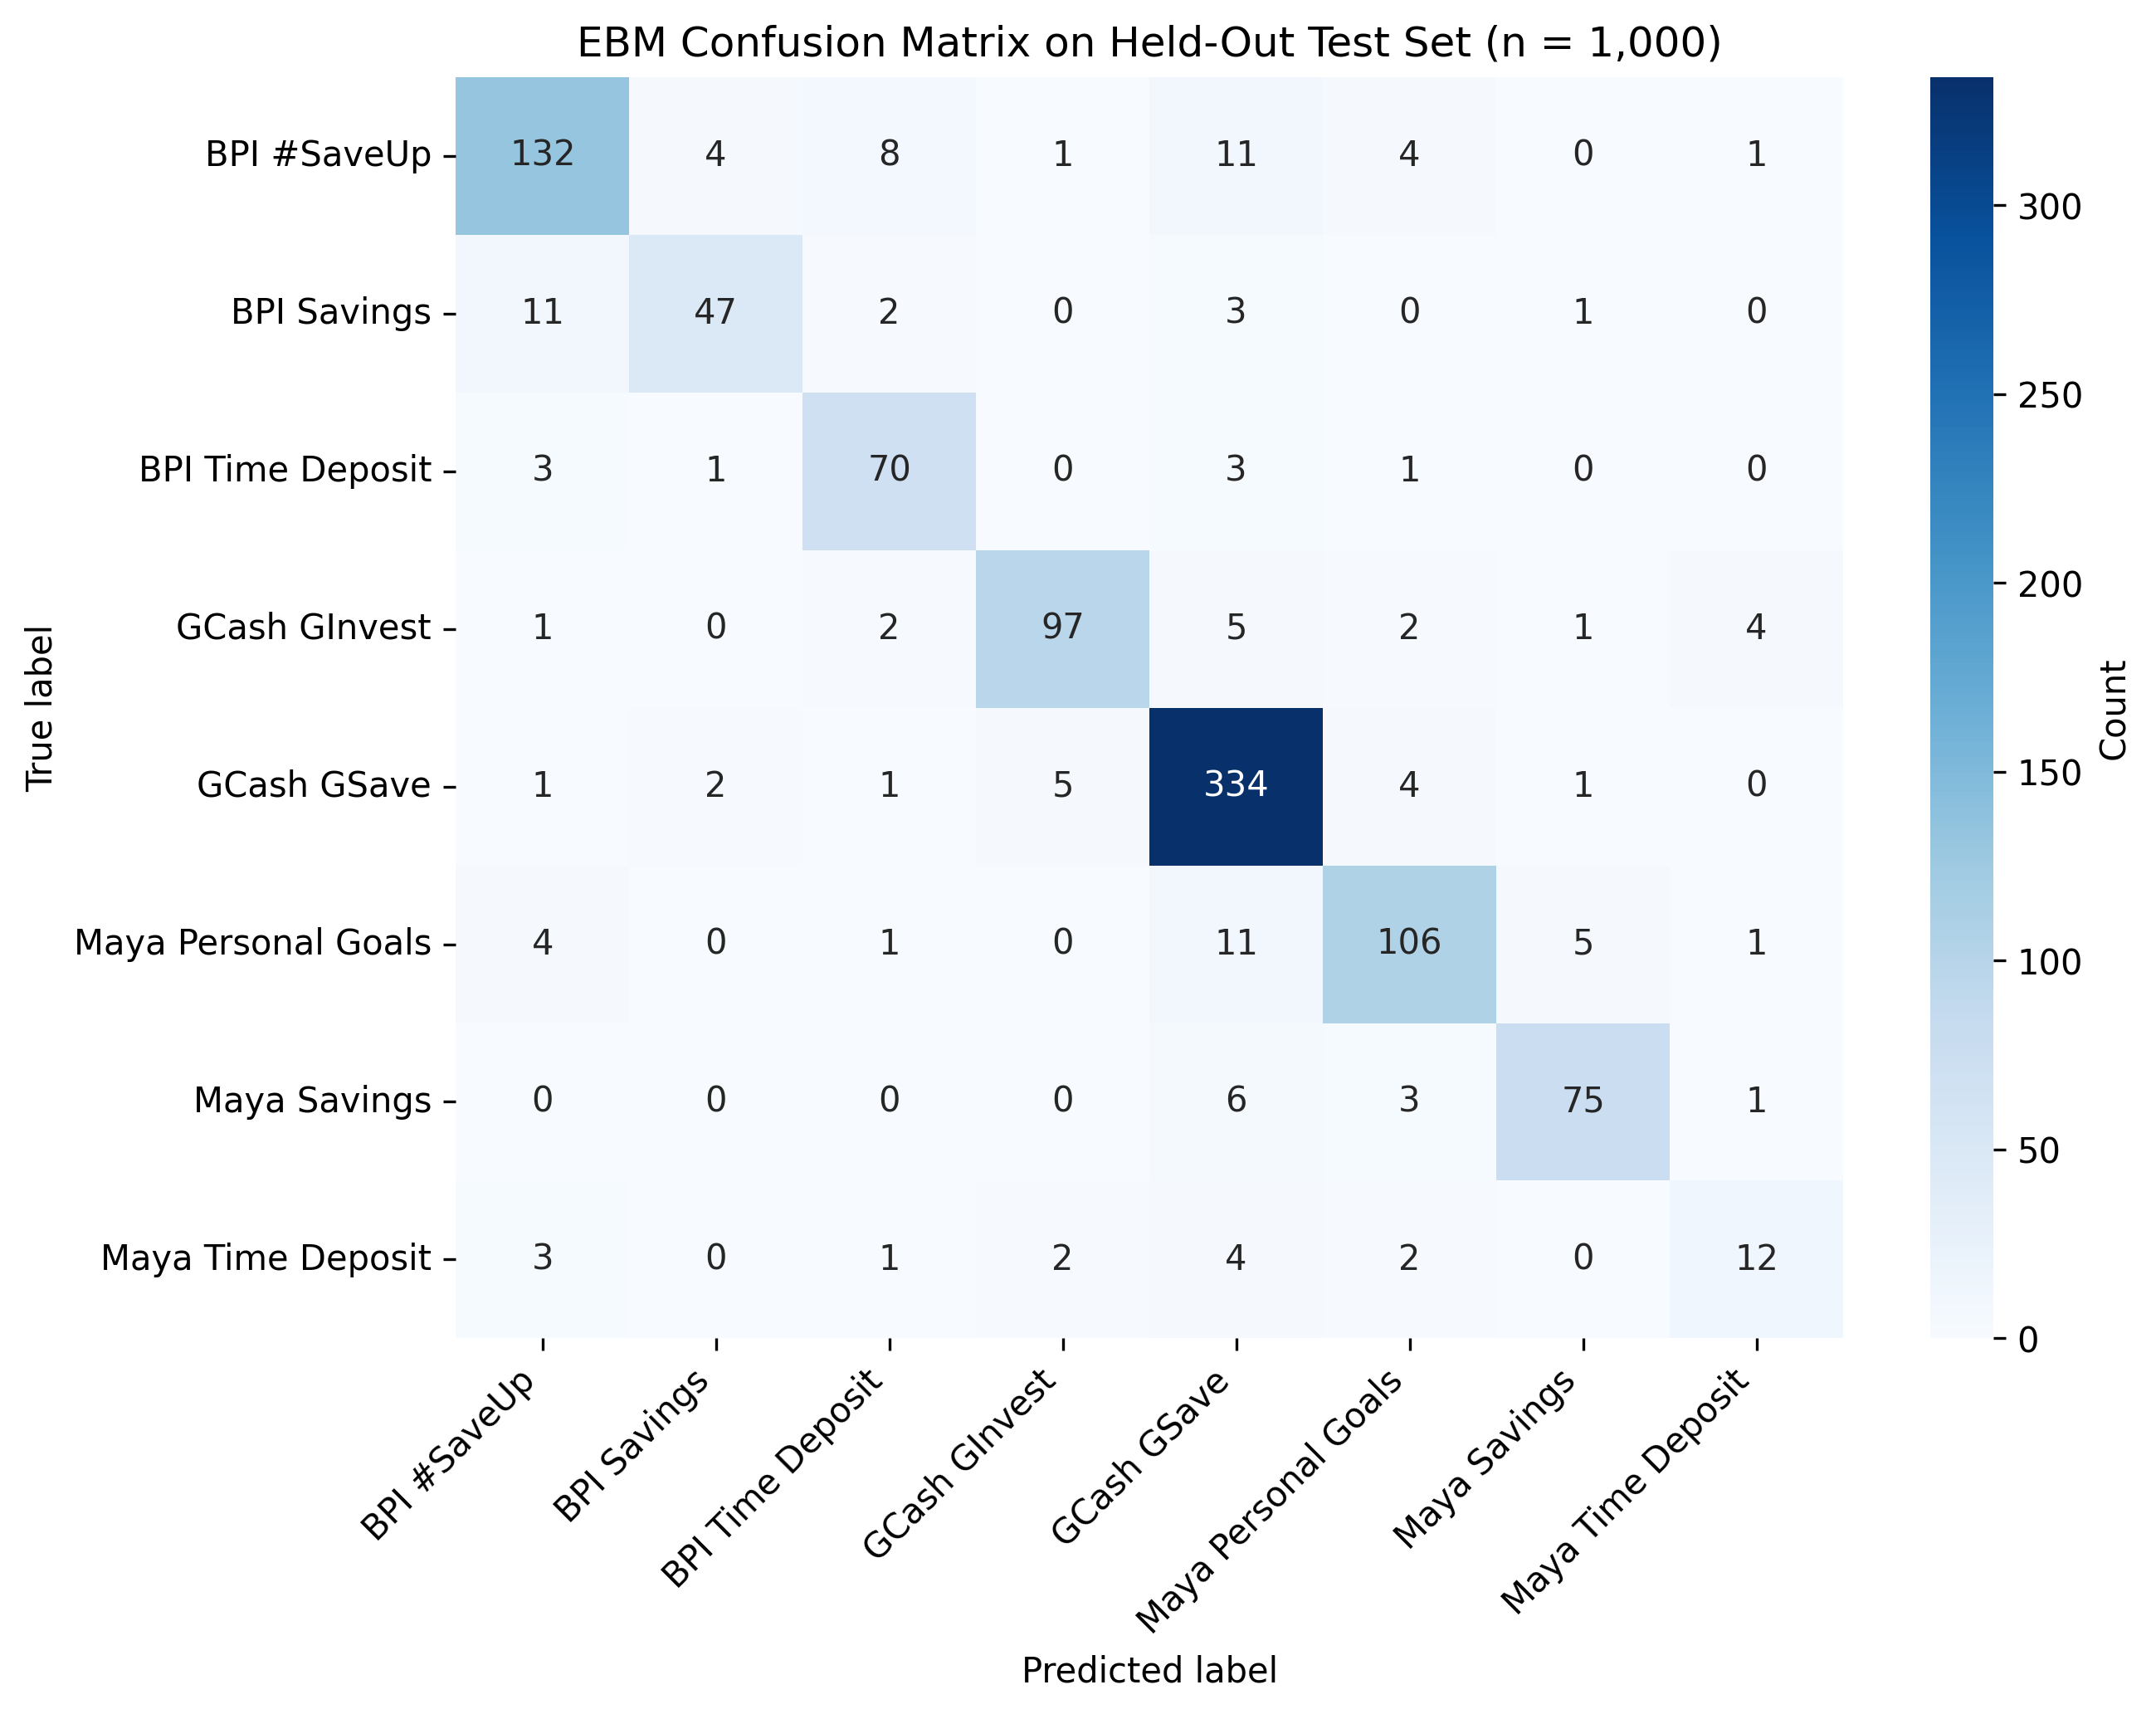
\includegraphics{cm_ebm.png}| and
    \verb|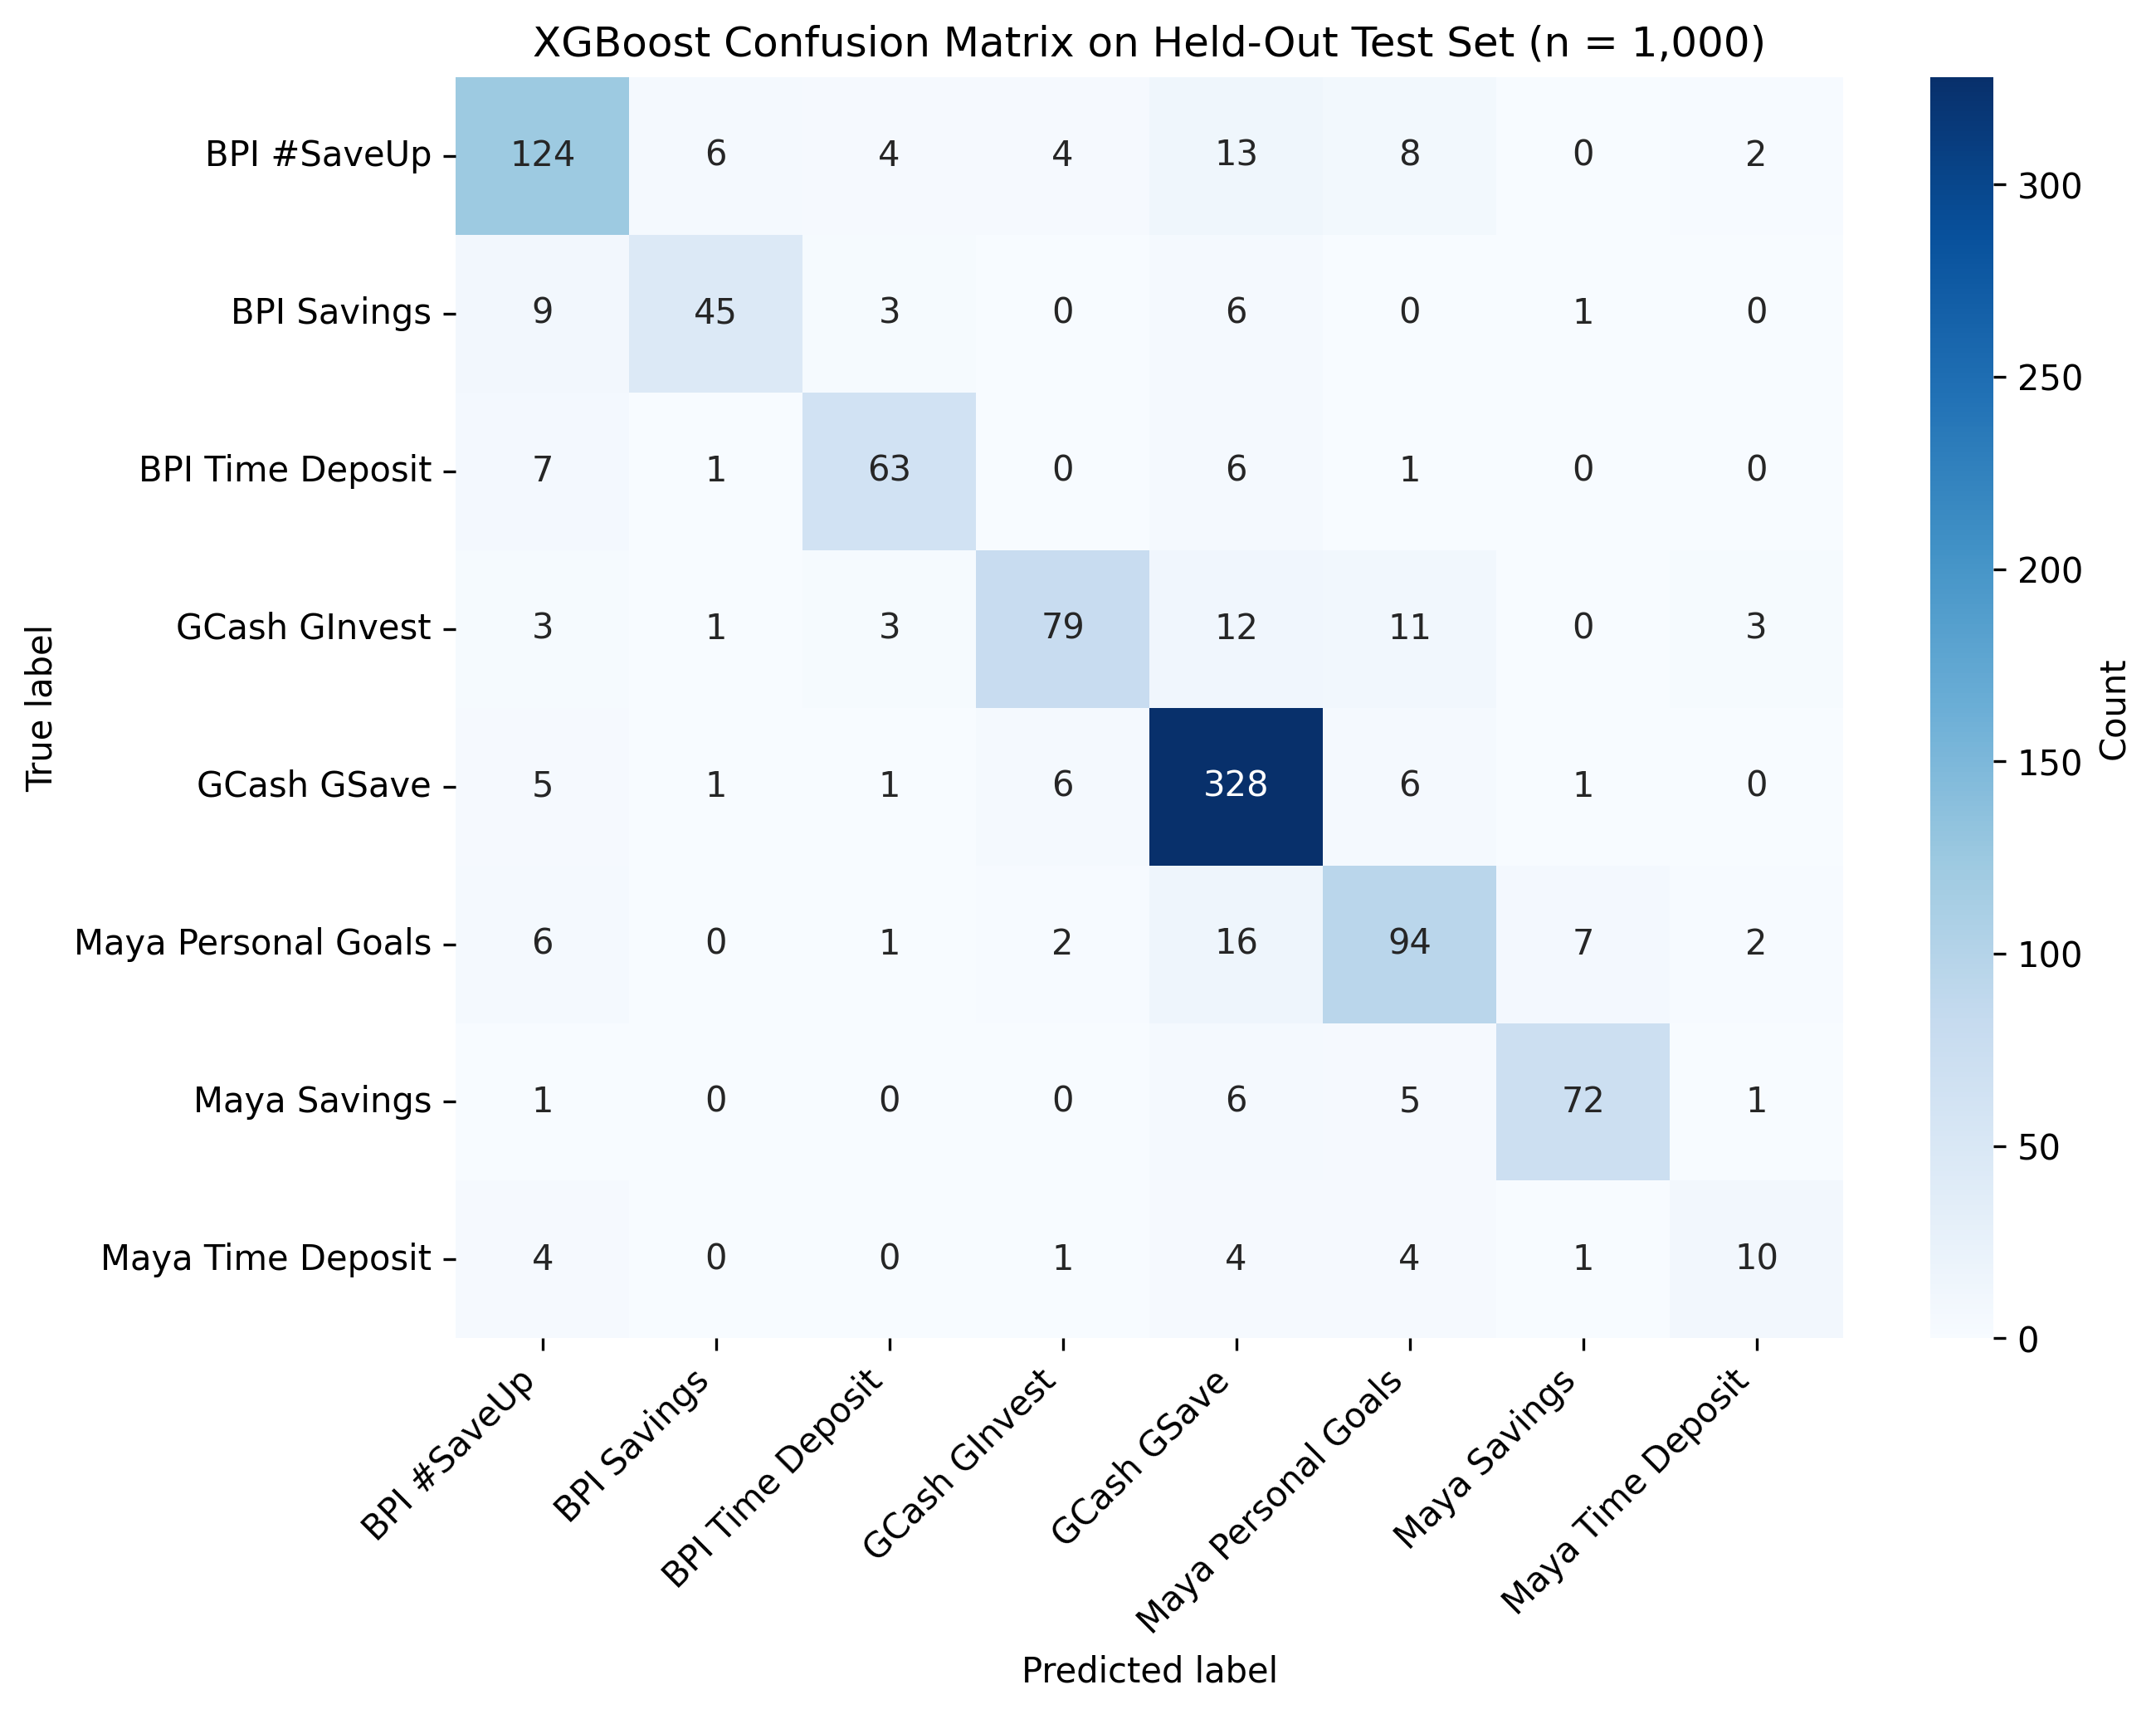
\includegraphics{cm_xgb.png}| calls in the paper resolve
    without a path prefix.
\end{itemize}

\subsection*{3.6 FastAPI backend}

\begin{itemize}
    \item \texttt{backend/main.py}: extended the \texttt{UserInput}
    Pydantic schema with \texttt{education}, \texttt{primary\_ewallet},
    and \texttt{receives\_remittance}, including validation rules and
    example values.
    \item \texttt{backend/explainability.py}:
    \begin{itemize}
        \item Added \texttt{primary\_ewallet} to \texttt{CONTROLLABLE\_CAT}
        so it can drive counterfactuals.
        \item Extended \texttt{VALID\_CATEGORIES} for
        \texttt{primary\_ewallet}.
        \item Extended \texttt{FEATURE\_LABELS} with human-readable
        labels for the three new fields.
        \item Added templated phrases in \texttt{\_describe\_feature}
        for \texttt{education}, \texttt{primary\_ewallet}, and
        \texttt{receives\_remittance}.
        \item Added a \texttt{primary\_ewallet}-specific
        \texttt{\_build\_counterfactual\_sentence}.
        \item Updated \texttt{\_preprocess} to accept the three new
        fields from raw user input.
    \end{itemize}
\end{itemize}

\subsection*{3.7 Next.js frontend}

\begin{itemize}
    \item \texttt{frontend/types/api.ts}: extended
    \texttt{RecommendRequest} with the three new fields and their
    string-literal types.
    \item \texttt{frontend/components/ProfileForm.tsx}:
    \begin{itemize}
        \item Updated \texttt{FormData} and \texttt{initialFormData}.
        \item Added a Select for \emph{Educational attainment} in
        Step~1 with validation in \texttt{isStepValid}.
        \item Modified the \emph{E-wallet} toggle to reset
        \texttt{primary\_ewallet} to \textsc{Neither} when toggled off,
        and added a conditional radio-style selector that appears when
        e-wallet is enabled.
        \item Added a toggle for \emph{Receives OFW remittance} in
        Step~2.
        \item Updated the payload construction in \texttt{handleSubmit}
        accordingly.
    \end{itemize}
\end{itemize}

\section*{4. Paper revisions (\texttt{SP2\_Matias\_journal.tex})}

\subsection*{4.1 Front matter}

\begin{itemize}
    \item \textbf{Abstract} rewritten to report 16 features, the new
    headline metrics (EBM weighted F1 $=0.8711$, AUC-ROC $=0.9761$,
    gaps $+5.93$ / $+0.90$ pp), and the cross-validation stability
    figure $0.870 \pm 0.006$.
    \item \textbf{Objectives \S I.C} and \textbf{Scope \S I.E} updated
    from ``13 features'' to ``16 features''; the source list was
    expanded to include the PSA 2020 Census.
\end{itemize}

\subsection*{4.2 Methodology (\S III)}

\begin{itemize}
    \item \S III.B sample-size paragraph: feature counts updated
    ($13 \to 16$ input; $17 \to 20$ total with derived).
    \item \S III.B.2 narrative paragraph: revised to introduce the
    three new features and explicitly note that they were added in
    response to defense-panel feedback.
    \item \textbf{Table~II (\texttt{tab:features})}: added three rows
    for \texttt{education}, \texttt{primary\_ewallet}, and
    \texttt{receives\_remittance} with PSA / BSP source citations.
    \item \textbf{Table~III (\texttt{tab:feat-outcome})}: added five
    rows covering the three new features' expected directions and
    products.
    \item \S III.E (Conditional Dependency DAG): extended with the
    three new conditional edges; ``Acrylic'' typo corrected to
    ``Acyclic.''
    \item \S III.E.4 (label-generation logic): rewritten to describe
    the eleven-dimension scoring system with the observable
    platform-attachment bonus replacing the previous hidden random
    one. Rule \textbf{R3} updated to require
    \texttt{primary\_ewallet} $\in$ \{Maya, Both\}; new rules \textbf{R9}
    (education) and \textbf{R10} (remittance) added.
    \item ``Four properties'' paragraph trimmed to remove the
    no-longer-applicable hidden-random-bonus argument.
\end{itemize}

\subsection*{4.3 Results and discussion (\S IV)}

\begin{itemize}
    \item \textbf{Table~V (\texttt{tab:desc-stats})}: added the
    \texttt{receives\_remittance} row.
    \item \S IV.A categorical-features paragraph: rewritten with new
    distributions (employment, education, location, primary e-wallet,
    savings goal, risk tolerance, investment horizon, remittance).
    \item \textbf{Table~VI (\texttt{tab:alignment})}: added rows for
    remittance recipients ($23.0\%$, within PSA FIES range), College+Graduate
    attainment ($38.4\%$), and the GCash:Maya $\sim$2:1 ratio; the
    surrounding paragraph was updated.
    \item \textbf{Table~VII (\texttt{tab:class-dist})}: refreshed with
    new counts; imbalance ratio now $14.4\times$ (vs.\ previous
    $7.3\times$). The accompanying paragraph was updated to explain
    the widened ratio in terms of \texttt{primary\_ewallet}.
    \item \textbf{Table~VIII (\texttt{tab:split})}: refreshed train/test
    counts.
    \item \S IV.B.2 (circular-reasoning paragraph): revised to
    reference the new $0.8711$ F1 and the residual on the smallest
    class (\texttt{maya\_time\_deposit} F1 $=0.5581$).
    \item \S IV.C.1 (training configuration): ``$17$-column'' updated
    to ``$20$-column''; ``five categoricals'' updated to ``seven
    categoricals'' with the categorical names listed.
    \item \textbf{Table~IX (\texttt{tab:ebm-hp})}:
    \texttt{feature\_names} entry updated from ``17 entries'' to ``20
    entries''.
    \item Cross-validation stability paragraph: rewritten with the new
    per-fold accuracies $\{0.868, 0.868, 0.860, 0.877, 0.877\}$, mean
    $0.870$, std $0.0064$, and a $\sim$0.5$\sigma$ test-vs-CV
    agreement.
    \item \textbf{Table~X (\texttt{tab:perf})}: refreshed with new
    metrics for both models; majority-class baseline recomputed
    (Accuracy $0.348$; F1 $0.180$).
    \item \textbf{Tables~XI--XII (per-class reports)}: rewritten from
    the new EBM and XGBoost classification reports.
    \item Per-class and confusion-matrix narrative paragraphs
    rewritten: the previously dominant
    \texttt{maya\_savings}$\to$\texttt{gcash\_gsave} confusion (117 of
    133) is now reduced to 6 of 85, with residual confusions clustering
    around \texttt{gcash\_gsave} as the highest-prior class.
    \item \S IV.C.3 (performance discussion) rewritten with new
    headlines, contextualization against West (binary credit-scoring,
    F1 0.70--0.85) and Bussmann et al.\ (explainable credit-risk
    accuracy 0.60--0.75), and a sentence linking the closer
    accuracy/AUC agreement to the
    \texttt{primary\_ewallet}-driven disambiguation.
    \item \textbf{Table~XIII (\texttt{tab:threshold})}: refreshed with
    $+5.93$ pp F1 gap and $+0.90$ pp AUC gap; surrounding paragraph
    updated.
    \item SHAP face-validity paragraph (\S III): updated to list
    \texttt{primary\_ewallet} as a top feature alongside income, risk
    tolerance, existing savings, and digital savviness.
\end{itemize}

\subsection*{4.4 Conclusion and recommendations (\S V)}

\begin{itemize}
    \item \textbf{Table~XIV (\texttt{tab:obj})}: all four objective
    rows refreshed with the new headline metrics and the resolution of
    the \texttt{maya\_savings} pathology.
    \item \S V.B Contribution~1 and Contribution~2: feature count and
    headline metrics updated; CV stability check explicitly cited.
    \item \S V.C: added \textbf{Recommendation~R4} (tuned-XGBoost
    benchmark and multi-seed replication), so the body's existing
    references to ``Recommendation~R4'' now resolve.
    \item \S V.D Closing Statement: updated with the new metrics.
\end{itemize}

\subsection*{4.5 Sweep verification}

A grep sweep was run for stale numeric strings (\texttt{0.6088},
\texttt{0.5839}, \texttt{0.9114}, \texttt{0.8917}, \texttt{0.6540},
\texttt{0.6040}, \texttt{+2.49}, \texttt{+1.97}, \texttt{0.0429},
\texttt{27.94}, \texttt{3.84}, \texttt{0.279}, \texttt{13 features},
\texttt{17 entries}). No matches were returned, confirming that no
prior-iteration number remains in the manuscript.

\section*{5. New files added today}

\begin{itemize}
    \item \texttt{cm\_ebm.png} (project root) --- regenerated EBM
    confusion-matrix figure.
    \item \texttt{cm\_xgb.png} (project root) --- regenerated XGBoost
    confusion-matrix figure.
    \item \texttt{financial\_advisor\_brief.tex} --- 2--3 page brief
    requesting expert review from a practising financial advisor (panel
    recommendation \#3). Compiles to a standalone PDF.
    \item \texttt{paper\_and\_code\_changelog.tex} --- this document.
\end{itemize}

\section*{6. Reproducibility checklist}

The full pipeline can be re-executed in order. All commands are run from
the project root:

\begin{enumerate}
    \item \texttt{python data/generate\_synthetic\_data.py}
    --- regenerates \texttt{data/synthetic\_filipino\_fintech.csv}.
    \item \texttt{python data/preprocess.py}
    --- regenerates \texttt{data/clean\_data.csv}.
    \item \texttt{python notebooks/train\_ebm.py}
    --- retrains the EBM and writes \texttt{models/ebm\_model.pkl},
    \texttt{models/label\_encoder.pkl}, and
    \texttt{models/model\_metadata.json}.
    \item \texttt{python notebooks/train\_model.py}
    --- retrains the XGBoost benchmark and writes
    \texttt{models/xgb\_model.pkl},
    \texttt{models/scaler.pkl}, \texttt{models/ordinal\_encoder.pkl}.
    \item \texttt{python notebooks/evaluate\_ebm\_for\_paper.py} and
    \texttt{python notebooks/evaluate\_xgb\_for\_paper.py}
    --- refresh \texttt{notebooks/paper\_ebm\_results.json} and
    \texttt{notebooks/paper\_results.json}.
    \item \texttt{python notebooks/ebm\_confusion-matrix.py} and
    \texttt{python notebooks/xgboost\_confusion-matrix.py}
    --- regenerate \texttt{cm\_ebm.png} and \texttt{cm\_xgb.png} (then
    copy to the project root next to the \texttt{.tex} file).
\end{enumerate}

A fixed seed (\texttt{random\_state=42}) is used at every stochastic
step, so re-execution should reproduce the numbers reported in the paper
to four decimal places.

\end{document}
